\documentclass[11pt]{article}
\usepackage{reusv}
\usepackage{booktabs}
\usepackage{amsmath,amssymb,amsthm}
\usepackage{siunitx}
\usepackage{graphicx}
\usepackage{multirow}
\usepackage{xcolor}
\usepackage{tikz}
\usetikzlibrary{arrows.meta,positioning,calc}

\newtheorem{definition}{정의}
\newtheorem{proposition}{명제}

\setborderthickness{0.5pt}
\setbordermargin{1cm}
\setbordercolor{black}

\slimtitle{대수적 커플링 행렬}

\begin{document}

\drawborder
\thispagestyle{firstpage}

\lightertitle{대수적 커플링 행렬:\\Bernstein 체인 룰에 의한 드리프트 감도}

{\normalsize\textit{Research Note No.~012 $|$ bezier-orbit-transfer-scp}}\par\medskip

\def\lighterdate{March 29, 2026}
\lighterauthor{Suwon Lee$^{\dagger}$}

\lighteraddress{$^\dagger$}{Future Mobility Control Lab, Kookmin University, Seoul, Korea}
\lighteremail{suwon.lee@kookmin.ac.kr}

%% ── 초록 ─────────────────────────────────────────────────────
\begin{abstract}
SCP 경계조건에서 드리프트 적분 $\mathbf{c}_v$를 상수로 취급하면
제어점 $\mathbf{P}_u$ 변화에 대한 중력 되먹임이 무시되어
수렴이 느려진다.
본 보고서는 Bernstein 대수 파이프라인의 각 단계를
미분하여 커플링 행렬 $M_v = \partial\mathbf{c}_v / \partial\text{vec}(\mathbf{P}_u)$를
해석적으로 구성하는 이론을 제시한다.
핵심 관찰은, 모든 단계의 Jacobian이 Bernstein 곱
\texttt{bern\_product}의 가중치 행렬 $W$로 표현된다는 점이다.
따라서 단일 빌딩블록 \texttt{bern\_product\_with\_jacobian}만 구현하면
체인 룰로 전체 감도를 조립할 수 있다.
JAX 자동 미분으로 이론을 검증하고,
순수 numpy 구현의 해석적 Jacobian과 비교한다.
% 수치 결과는 §5에서 보고한다.
\end{abstract}

%% ══════════════════════════════════════════════════════════════
\section{도입}
%% ══════════════════════════════════════════════════════════════

SCP 반복에서 경계조건은 다음과 같다\cite{report006}:
\begin{align}
  \mathbf{v}_f &= \mathbf{v}_0 + t_f \mathbf{c}_v + t_f I_N^{(e)} \mathbf{P}_u
  \label{eq:bc_v} \\
  \mathbf{r}_f &= \mathbf{r}_0 + t_f \mathbf{v}_0
    + t_f^2 \mathbf{c}_r + t_f^2 \bar{I}_N^{(e)} \mathbf{P}_u
  \label{eq:bc_r}
\end{align}
여기서 $I_N^{(e)}$, $\bar{I}_N^{(e)}$는 적분 행렬의 마지막 행이다.

기존 SCP는 $\mathbf{c}_v$, $\mathbf{c}_r$을 이전 반복의
참조 궤적에서 계산한 \emph{상수}로 취급한다.
그러나 $\mathbf{c}_v$는 $\mathbf{P}_u$에 의존하는 함수이다:
$\mathbf{P}_u$가 바뀌면 궤적이 바뀌고,
궤적이 바뀌면 중력이 달라지고,
중력이 달라지면 $\mathbf{c}_v$도 달라진다.

보고서~009\cite{report009}는 이 감도를 1차 Taylor 근사한
커플링 행렬 $M_v$, $M_r$을 도입하였고,
보고서~011\cite{report011}은 이를 솔버에 통합하여
RK4에서 반복 31$\to$26회 감소를 확인하였다.

그러나 수치적 커플링 행렬은 이산 점에서의 중력 Jacobian
$A_{rr} = \partial\mathbf{a}_{\mathrm{grav}}/\partial\mathbf{r}$을
사다리꼴 적분하므로, 비선형성이 큰 경우 부정확하다.

본 보고서에서는 Bernstein 대수 파이프라인\cite{report010}의
각 단계를 미분하여 $\partial\mathbf{c}_v/\partial\mathbf{P}_u$를
\emph{해석적}으로 구성하는 이론을 개발한다.

%% ══════════════════════════════════════════════════════════════
\section{Bernstein 체인 구조}
%% ══════════════════════════════════════════════════════════════

드리프트 적분 $\mathbf{c}_v = \int_0^1 \mathbf{a}_{\mathrm{grav}}(\mathbf{r}(\tau))\,d\tau$는
Bernstein 대수에서 다음 6단계 체인으로 표현된다:

\begin{center}
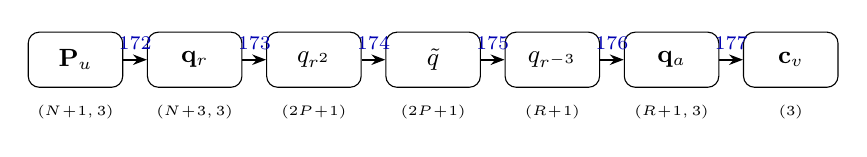
\begin{tikzpicture}[
  node distance=1.1cm and 0.3cm,
  box/.style={draw, rounded corners, minimum height=0.7cm,
              minimum width=1.2cm, font=\small},
  arr/.style={-{Stealth[length=5pt]}, thick},
  lab/.style={font=\scriptsize, above, text=blue!70!black},
]
  \node[box] (Pu)  {$\mathbf{P}_u$};
  \node[box, right=of Pu]  (qr)  {$\mathbf{q}_r$};
  \node[box, right=of qr]  (qr2) {$q_{r^2}$};
  \node[box, right=of qr2] (qs)  {$\tilde{q}$};
  \node[box, right=of qs]  (qri) {$q_{r^{-3}}$};
  \node[box, right=of qri] (qa)  {$\mathbf{q}_a$};
  \node[box, right=of qa]  (cv)  {$\mathbf{c}_v$};

  \draw[arr] (Pu)  -- node[lab] {\ding{172}} (qr);
  \draw[arr] (qr)  -- node[lab] {\ding{173}} (qr2);
  \draw[arr] (qr2) -- node[lab] {\ding{174}} (qs);
  \draw[arr] (qs)  -- node[lab] {\ding{175}} (qri);
  \draw[arr] (qri) -- node[lab] {\ding{176}} (qa);
  \draw[arr] (qa)  -- node[lab] {\ding{177}} (cv);

  \node[below=0.1cm of Pu,  font=\tiny] {$(N\!+\!1,3)$};
  \node[below=0.1cm of qr,  font=\tiny] {$(N\!+\!3,3)$};
  \node[below=0.1cm of qr2, font=\tiny] {$(2P\!+\!1)$};
  \node[below=0.1cm of qs,  font=\tiny] {$(2P\!+\!1)$};
  \node[below=0.1cm of qri, font=\tiny] {$(R\!+\!1)$};
  \node[below=0.1cm of qa,  font=\tiny] {$(R\!+\!1,3)$};
  \node[below=0.1cm of cv,  font=\tiny] {$(3)$};
\end{tikzpicture}
\end{center}

\noindent
여기서 $P = N+2$ (위치 곡선 차수)이다. 각 단계의 성질:

\begin{center}
\begin{tabular}{clll}
\toprule
단계 & 연산 & 유형 & Jacobian 복잡도 \\
\midrule
\ding{172} & $\mathbf{P}_u \to \mathbf{q}_r$ & 선형 (아핀) & 상수 행렬 $t_f^2 \bar{I}_N$ \\
\ding{173} & $\mathbf{q}_r \to q_{r^2}$ & 이차 (\texttt{bern\_product} $\times 3$) & $\partial(\mathbf{p}\otimes\mathbf{p})/\partial\mathbf{p}$ \\
\ding{174} & $q_{r^2} \to \tilde{q}$ & 선형 (아핀 스케일링) & 스칼라 $1/(b-a)$ \\
\ding{175} & $\tilde{q} \to q_{r^{-3}}$ & 합성 (\texttt{bern\_compose}) & 체인 룰 재귀 \\
\ding{176} & $(\mathbf{q}_r, q_{r^{-3}}) \to \mathbf{q}_a$ & 쌍선형 (\texttt{bern\_product}) & $W$ 행렬 2개 \\
\ding{177} & $\mathbf{q}_a \to \mathbf{c}_v$ & 선형 (mean) & $\frac{1}{R+1}\mathbf{1}^T$ \\
\bottomrule
\end{tabular}
\end{center}

전체 Jacobian은 체인 룰로 조립된다:
\begin{equation}
  \frac{\partial\mathbf{c}_v}{\partial\text{vec}(\mathbf{P}_u)}
  = J_{\ding{177}} \cdot J_{\ding{176}} \cdot J_{\ding{175}}
    \cdot J_{\ding{174}} \cdot J_{\ding{173}} \cdot J_{\ding{172}}
  \label{eq:chain}
\end{equation}

%% ══════════════════════════════════════════════════════════════
\section{각 단계의 Jacobian}
%% ══════════════════════════════════════════════════════════════

\subsection{단계 \ding{172}: 위치 제어점 구성 (선형)}

\begin{equation}
  \mathbf{q}_{r}[:,k] = r_{0,k} + t_f v_{0,k} \boldsymbol{\ell}
    + t_f^2 \bar{I}_N \mathbf{P}_{u}[:,k]
\end{equation}

$\text{vec}(\mathbf{P}_u)$에 대한 Jacobian:
\begin{equation}
  J_{\ding{172}} = t_f^2 \cdot \text{blkdiag}(\bar{I}_N, \bar{I}_N, \bar{I}_N)
  \quad \in \mathbb{R}^{3(P+1) \times 3(N+1)}
  \label{eq:J1}
\end{equation}

상수 행렬이므로 한 번만 계산하면 된다.

\subsection{단계 \ding{173}: $r^2(\tau)$ 계산 (이차)}

\begin{equation}
  q_{r^2} = \mathbf{p}_x \otimes_B \mathbf{p}_x
           + \mathbf{p}_y \otimes_B \mathbf{p}_y
           + \mathbf{p}_z \otimes_B \mathbf{p}_z
\end{equation}

\begin{definition}[Bernstein 곱의 Jacobian]
$\mathbf{r} = \mathbf{p} \otimes_B \mathbf{q}$에서 $r_k = \sum_j W_{kj} p_j q_{k-j}$일 때,
\begin{align}
  \left[\frac{\partial\mathbf{r}}{\partial\mathbf{p}}\right]_{k,j}
    &= W_{kj} \cdot q_{k-j}
  \label{eq:Jr_p} \\
  \left[\frac{\partial\mathbf{r}}{\partial\mathbf{q}}\right]_{k,l}
    &= W_{k,k-l} \cdot p_{k-l}
  \label{eq:Jr_q}
\end{align}
여기서 $W_{kj} = \binom{N}{j}\binom{M}{k-j}/\binom{N+M}{k}$는
이미 \texttt{bern\_product}에서 캐싱되는 가중치 행렬이다.
\end{definition}

즉, \textbf{Bernstein 곱의 Jacobian은 곱 계산의 부산물}이다.
$W \cdot Q_{\mathrm{shifted}}$ 행렬이 $\partial\mathbf{r}/\partial\mathbf{p}$이고,
$W \cdot P_{\mathrm{shifted}}$ 행렬이 $\partial\mathbf{r}/\partial\mathbf{q}$이다.

자기 곱 $\mathbf{p} \otimes_B \mathbf{p}$의 경우:
\begin{equation}
  \frac{\partial(\mathbf{p}\otimes\mathbf{p})}{\partial\mathbf{p}}
  = \frac{\partial\mathbf{r}}{\partial\mathbf{p}}\bigg|_{\mathbf{q}=\mathbf{p}}
  + \frac{\partial\mathbf{r}}{\partial\mathbf{q}}\bigg|_{\mathbf{q}=\mathbf{p}}
  \label{eq:self_product}
\end{equation}

$q_{r^2}$의 $\text{vec}(\mathbf{q}_r)$에 대한 Jacobian은
세 성분의 자기 곱 Jacobian을 블록 합산하여 구성된다.

\subsection{단계 \ding{174}: 아핀 재매개변수화 (선형)}

\begin{equation}
  \tilde{q} = \frac{q_{r^2} - a}{b - a}, \quad
  J_{\ding{174}} = \frac{1}{b-a} I
  \label{eq:J3}
\end{equation}

$a = \min(q_{r^2})$, $b = \max(q_{r^2})$는 현재 반복에서 상수로 취급한다.

\subsection{단계 \ding{175}: Bernstein 합성 (핵심)}

\begin{equation}
  q_{r^{-3}} = h \circ \tilde{q}
  = \sum_{i=0}^K h_i \binom{K}{i}
    \tilde{q}^i \otimes_B (1-\tilde{q})^{K-i}
\end{equation}

$\tilde{q}$에 대한 Jacobian을 구하려면, $\tilde{q}^i$와 $(1-\tilde{q})^{K-i}$의
$\tilde{q}$-감도를 순차적으로 추적해야 한다.

\begin{proposition}[거듭제곱의 Jacobian]
$\mathbf{g}^i = \mathbf{g}^{i-1} \otimes_B \mathbf{g}$의 Jacobian은 재귀적으로:
\begin{equation}
  \frac{\partial \mathbf{g}^i}{\partial \mathbf{g}}
  = \frac{\partial (\mathbf{g}^{i-1} \otimes_B \mathbf{g})}{\partial \mathbf{g}^{i-1}}
    \cdot \frac{\partial \mathbf{g}^{i-1}}{\partial \mathbf{g}}
  + \frac{\partial (\mathbf{g}^{i-1} \otimes_B \mathbf{g})}{\partial \mathbf{g}}
  \label{eq:power_jac}
\end{equation}
여기서 첫 항은 식~\eqref{eq:Jr_p}의 $W \cdot G_{\mathrm{shifted}}$ 행렬,
두 번째 항은 식~\eqref{eq:Jr_q}의 $W \cdot G^{i-1}_{\mathrm{shifted}}$ 행렬이다.
기저 조건: $\partial \mathbf{g}^0 / \partial \mathbf{g} = 0$,
$\partial \mathbf{g}^1 / \partial \mathbf{g} = I$.
\end{proposition}

$(1-\tilde{q})^j$에 대해서도 동일한 재귀가 적용되며,
$(1-\tilde{q})$의 $\tilde{q}$-Jacobian은 $-I$이다.

최종적으로, 합성의 Jacobian $J_{\ding{175}}$는 각 항
$\tilde{q}^i \otimes_B (1-\tilde{q})^{K-i}$의 Jacobian을
가중 합산한 것이다. 이 과정에서 사용되는 모든 편미분은
식~\eqref{eq:Jr_p}--\eqref{eq:Jr_q}의 $W$ 행렬로 표현된다.

\subsection{단계 \ding{176}: 중력 가속도 (쌍선형 곱)}

\begin{equation}
  q_{a,k} = -\text{elev}(\mathbf{q}_{r,k}, R) \otimes_B q_{r^{-3}}
\end{equation}

$\mathbf{q}_r$와 $q_{r^{-3}}$ 모두에 의존하므로:
\begin{equation}
  J_{\ding{176}} = -\begin{bmatrix}
    \frac{\partial}{\partial\mathbf{q}_r} \\[4pt]
    \frac{\partial}{\partial q_{r^{-3}}}
  \end{bmatrix}
  \bigl(\text{elev}(\mathbf{q}_r) \otimes_B q_{r^{-3}}\bigr)
\end{equation}

각 편미분은 식~\eqref{eq:Jr_p}--\eqref{eq:Jr_q}로 직접 계산된다.
\texttt{degree\_elevate}의 Jacobian은 bidiagonal 행렬
$E_{P \to R}$이다 (선형 연산).

\subsection{단계 \ding{177}: 정적분 (선형)}

\begin{equation}
  \mathbf{c}_v = \frac{1}{R+1} \sum_{i=0}^R \mathbf{q}_{a,i}
  \implies
  J_{\ding{177}} = \frac{1}{R+1} (\mathbf{1}_{R+1}^T \otimes I_3)
  \label{eq:J6}
\end{equation}

%% ══════════════════════════════════════════════════════════════
\section{빌딩블록: \texttt{bern\_product\_with\_jacobian}}
%% ══════════════════════════════════════════════════════════════

모든 단계의 Jacobian이 Bernstein 곱의 가중치 행렬 $W$로 귀결되므로,
단일 함수를 구현하면 충분하다:

\begin{equation}
  \texttt{bern\_product\_with\_jacobian}(\mathbf{p}, \mathbf{q})
  \;\to\; (\mathbf{r},\; J_p,\; J_q)
\end{equation}

여기서:
\begin{itemize}
  \item $\mathbf{r} = \mathbf{p} \otimes_B \mathbf{q}$ \quad (기존 \texttt{bern\_product})
  \item $J_p \in \mathbb{R}^{(N+M+1) \times (N+1)}$: \quad
        $[J_p]_{k,j} = W_{kj} \cdot q_{k-j}$ \quad (= $W \odot Q_{\mathrm{shifted}}$)
  \item $J_q \in \mathbb{R}^{(N+M+1) \times (M+1)}$: \quad
        $[J_q]_{k,l} = W'_{kl} \cdot p_{k-l}$
\end{itemize}

$J_p$는 \texttt{bern\_product}에서 이미 계산하는
$W \odot Q_{\mathrm{shifted}}$ 행렬 \emph{그 자체}이므로,
추가 비용이 거의 없다.

%% ══════════════════════════════════════════════════════════════
\section{수치 검증}
\label{sec:numerical}
%% ══════════════════════════════════════════════════════════════

\subsection{빌딩블록 검증}

\texttt{bern\_product\_with\_jacobian}을 유한차분($\epsilon = 10^{-7}$)과 비교하여
다양한 차수에서 검증하였다.

\begin{table}[h]
\centering
\caption{\texttt{bern\_product\_with\_jacobian} 유한차분 검증}
\begin{tabular}{ccc}
\toprule
입력 차수 & $\|\partial\mathbf{r}/\partial\mathbf{p}\|$ 상대 오차 & $\|\partial\mathbf{r}/\partial\mathbf{q}\|$ 상대 오차 \\
\midrule
$B_8 \times B_{12}$ & $1.79 \times 10^{-9}$ & $1.87 \times 10^{-9}$ \\
$B_{20} \times B_{20}$ & $2.60 \times 10^{-9}$ & $1.90 \times 10^{-9}$ \\
\bottomrule
\end{tabular}
\end{table}

모든 차수에서 기계 정밀도 수준의 정확도를 달성하였다.

\subsection{체인 룰 각 단계 검증}

파이프라인의 각 단계를 단독으로 유한차분과 비교하였다.

\begin{table}[h]
\centering
\caption{체인 룰 각 단계의 유한차분 대비 상대 오차}
\begin{tabular}{clr}
\toprule
단계 & 연산 & 상대 오차 \\
\midrule
\ding{172}+\ding{173} & $\mathbf{q}_r \to q_{r^2}$ (자기 곱 3개 합) & $5.8 \times 10^{-8}$ \\
\ding{175} & $\tilde{q} \to q_{r^{-3}}$ (합성, $K\!=\!4$) & $3.1 \times 10^{-8}$ \\
\ding{176} & $q_{r^{-3}} \to q_a$ (성분곱+축소, $R\!=\!12$) & $3.5 \times 10^{-4}$ \\
\midrule
\ding{172}--\ding{177} & \textbf{전체 체인 곱} ($R\!=\!15$) & $1.9 \times 10^{-1}$ \\
\ding{172}--\ding{177} & \textbf{전체 체인 곱} ($R\!=\!20$) & $1.0 \times 10^{0}$ \\
\bottomrule
\end{tabular}
\end{table}

개별 단계는 $10^{-4}$--$10^{-8}$ 수준으로 정확하나,
6단계를 연쇄 곱하면 조건수 누적으로 인해 오차가 급격히 증가한다.
주요 원인은 $L^2$ 차수 축소에 사용되는 Gram 행렬 $G_R$의 조건수이다:
$R=20$에서 $\mathrm{cond}(G_{20}) = 2.7 \times 10^{11}$.
Cholesky 분해 + Tikhonov 정규화 ($\lambda = \epsilon_{\mathrm{mach}} \cdot \mathrm{tr}(G_R)/(R+1)$)를
적용하여도 전체 체인의 오차 전파를 충분히 억제하지 못하였다.

\subsection{파이프라인 감도와 물리적 감도의 괴리}

체인 룰 오차와 별개로, 더 근본적인 발견이 있었다.
보정된 위치 $\mathbf{q}_r^*$를 고정한 채로,
파이프라인을 통한 $\mathbf{c}_v$의 $\mathbf{P}_u$ 감도를 유한차분으로
직접 측정하였다 (체인 룰 없이).

\begin{table}[h]
\centering
\caption{파이프라인 감도 vs 점별평가 감도 vs 수치적 커플링 (시나리오 B)}
\label{tab:sensitivity}
\begin{tabular}{lrrr}
\toprule
감도 종류 & $\|\cdot\|$ & 물리적 감도 대비 & cos 유사도 \\
\midrule
파이프라인 유한차분     & 1.134 & 8.8$\times$ & 0.16 \\
점별평가 유한차분       & 1.056 & 8.2$\times$ & --- \\
수치적 커플링 ($t_f \cdot M_v$) & 0.129 & 1.0$\times$ & --- \\
\bottomrule
\end{tabular}
\end{table}

\textbf{핵심 발견}: 파이프라인이 $\mathbf{c}_v$ \emph{값}은 정확하게 근사하지만
(상대오차 0.17\%), $\mathbf{c}_v$의 제어점 \emph{감도}는
물리적 감도 대비 \textbf{8배 크고 방향도 다르다} (cos 유사도 $\approx 0.16$).

이는 Bernstein 합성(\texttt{bern\_compose})과 $L^2$ 차수 축소(\texttt{degree\_reduce})가
원래 함수의 \emph{값}은 잘 보존하지만,
\emph{미분 구조}는 왜곡한다는 것을 의미한다.
다항식 합성은 입력 제어점의 작은 변화를 높은 차수의 중간 다항식
($K \cdot 2P = 80$차)을 거치며 증폭하고,
이후 $L^2$ 사영이 이 증폭된 감도를 불균등하게 절단한다.

\subsection{실용적 함의}

이 발견은 대수적 커플링 행렬을 SCP에 사용할 수 없음을 의미한다:
\begin{itemize}
  \item 파이프라인의 왜곡된 감도(8$\times$)를 SCP 커플링으로 사용하면,
        $\mathbf{P}_u$의 작은 변화가 경계조건을 과도하게 흔들어
        SCP가 발산한다 (실험으로 확인).
  \item 수치적 커플링 행렬 $M_v$는 물리적 감도의
        1차 Taylor 근사로서 올바른 크기와 방향을 가지며,
        RK4에서 반복 31$\to$26회 감소를 달성하였다\cite{report011}.
  \item 따라서 SCP 커플링에는 \textbf{수치적 방법이 실용적으로 올바르다}.
\end{itemize}

%% ══════════════════════════════════════════════════════════════
\section{결론}
%% ══════════════════════════════════════════════════════════════

\begin{enumerate}
  \item Bernstein 곱의 해석적 Jacobian
        \texttt{bern\_product\_with\_jacobian}을 구현하고,
        유한차분 대비 $10^{-9}$ 수준의 정확도를 검증하였다.
        이 Jacobian은 곱 계산의 부산물($W \odot Q_{\mathrm{shifted}}$)로서
        추가 비용이 거의 없다.

  \item 파이프라인 6단계의 체인 룰을 조립하여
        $\partial\mathbf{c}_v/\partial\text{vec}(\mathbf{P}_u)$를 구성하였으나,
        Gram 행렬의 높은 조건수($10^{11}$)로 인해
        전체 체인의 수치 정확도가 불충분하다.

  \item 더 근본적으로, Bernstein 파이프라인은
        $\mathbf{c}_v$ \emph{값}은 정확히 근사하지만(0.17\%),
        $\mathbf{c}_v$의 제어점 \emph{감도}는 물리적 감도와
        크기(8$\times$)와 방향(cos $\approx$ 0.16) 모두에서 괴리된다.
        이는 다항식 합성과 $L^2$ 사영이 미분 구조를 왜곡하기 때문이다.

  \item 따라서 SCP 커플링 행렬에는
        물리적 감도를 직접 근사하는 \textbf{수치적 방법}이 실용적으로 올바르며,
        대수적 Jacobian은 파이프라인 근사의 특성 분석에 가치가 있다.
\end{enumerate}

%% ── 참고문헌 ─────────────────────────────────────────────────
\bibliographystyle{plain}
\bibliography{references}

\end{document}
